\documentclass[11pt]{article}

\usepackage[utf8]{inputenc}
\usepackage[brazil]{babel}
\usepackage[section]{placeins} 
\usepackage{graphicx}
\usepackage{hyperref}

\begin{document}
\title{TerraCota}
\author{NullPointer Corporation}
\date{}
\maketitle

\newpage

\tableofcontents
\newpage
\section{Apresentação}
TerraCota é um jogo do tipo aventura com uso de \textit{puzzles} para progresso na história do jogo.  O protagonista irá se comunicar com os habitantes das torres através de símbolos, os quais devem ser traduzidos para cumprir os objetivos das missões.

\section{Resumo do jogo}
Por conta de um desastre iminente, a humanidade construiu diversas torres autossuficientes para se abrigar.
Centenas de anos depois, o mundo já reequilibrado, a sociedade \lq\lq evoluiu\rq\rq\ e passou a falar por meio de símbolos, ao invés de sons e palavras, e retornou às culturas de seus ancestrais.

Em uma das torres vive Inti, em uma sociedade que esqueceu da existência do mundo exterior.  Um dia, por algum motivo, ele acaba encontrando a saída da torre, e ao descobrir que existe algo além da torre, decide explorar.

Ele encontra Killa sentada nos galhos de uma árvore, e ela misteriosamente possui um interesse grande por ele.

\section{Principais Características}
Uma das características mais interessantes do jogo é o modo como os gêneros aventura e puzzle interagem entre si, fazendo com o que o jogador precise pensar e decifrar qual será sua missão, pois as informações serão dadas através de símbolos.

A movimentação do personagem, baseada em jogos \textit{Beat 'em Up}, também é uma característica diferenciada do jogo, pois traz um modo de exploração em visão em múltiplos planos. A inspiração desse estilo de movimentação veio, principalmente, do jogos Capitão Comando, Little Fighter 2 e Double Dragon.

\section{Público}
A classificação do jogo será E10+, pois o personagem terá inimigos para combater durante os níveis.

\section{Plataformas alvo}
As plataformas suportadas, inicialmente, serão Windows e Linux.
O Linux possui um grande suporte de bibliotecas e ferramentas de desenvolvimento de software e o Windows possui uma grande base de usuários jogadores, fazendo com que ambas os sistemas operacionais se tornem alvos para o jogo.

\section{Logotipos}
\subsection{Logotipo do jogo}
\begin{figure}[!htp]
\centering
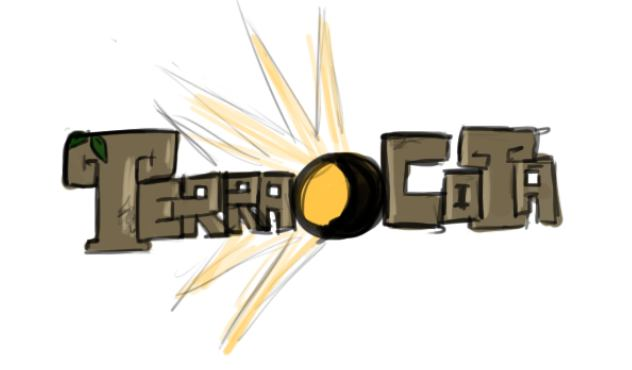
\includegraphics[scale=0.75]{logo-terracota.jpg}
\caption{Logo do jogo TerraCota}
\label{TerraCota logo}
\end{figure}

\subsection{Logotipo das tecnologias envolvidas}
\begin{figure}[!htp]
\centering

\includegraphics[scale=0.75]{logo-vim.png}
\caption{Editor de Texto Vim}
\label{Vim logo}
\end{figure}

\begin{figure}[!htp]
\centering

\includegraphics[scale=0.75]{logo-sublime-text.png}
\caption{Editor de Texto Sublime Text}
\label{Sublime Text logo}
\end{figure}

\begin{figure}[!htp]
\centering

\includegraphics[scale=0.75]{logo-gnu-linux.png}
\caption{Sistema Operacional GNU/Linux}
\label{GNU/Linux logo}
\end{figure}

\begin{figure}[!htp]
\centering

\includegraphics[scale=0.75]{logo-sdl.png}
\caption{Biblioteca para desenvolvimento Simple DirectMedia Layer}
\label{SDL logo}
\end{figure}

\section{Equipe}
\subsection{Contato por e-mail}
A equipe pode ser contatada através do email: \url{nullpointercorporation@gmail.com}

\subsection{Contato por repositório}
Caso a intenção seja contatar a equipe para reportar algum \textit{bug} no jogo, o endereço será: \url{https://github.com/nullpointercorporation/terracota/issues/}
\newpage
\end{document}

